    \chapter{Experimental Design}
    \label{ch:experiment}
    \thispagestyle{fancy}

    To empirically answer the questions posed in the introductory chapter and to test the theoretical statements of the model described in chapter \ref{ch:model}, I designed and conducted a laboratory experiment. The current chapter explains the experimental design and begins with a general overview in section \ref{sec:gen_str}. It then addresses the considerations going into the selection, design and parametrization of the Real Effort Task (RET) in section \ref{sec:RET}, and details in section \ref{sec:intro_exp} each element of the experiment. In order to make explicit which information was available to players at each stage of the procedure, each component of the experiment is shown with its respective screenshots in the chronological order in which they were presented to participants.\\
    
    The treatment intervention is explained in subsection \ref{sec:treat}, while the hypotheses derived from the research questions proposed in the introduction chapter are laid out formally in the context of this specific design in section \ref{sec:hyp}.
    
\section{General Structure of the Experiment}
\label{sec:gen_str}
    
    The general goal in the experiment is to let players invest their earnings from solving a Real Effort Task to increase their individual chances of winning a contest that awards the double wage in the following round, as explained in the theoretical model of section \ref{ch:model}. This process is repeated several times in groups that remain constant throughout the trial.\\ 
    
    % To avoid having a situation where wage increase does not result in effort increase, paid leisure is introduced. How paid leisure works is explained in detail in subsection \ref{ss:switch_mode}.\\

    The experiment is roughly divided into three sections as shown in Figure \ref{fig:exp_str}.\footnote{ Table \ref{tab:exp_design} in the appendix lists a detailed breakup of the three main sections and its contents.} The first is an introductory section where the principal components of the experiment, including the RET, are explained in great detail to the participants. In this first section, participants are also asked several control questions to test their understanding of the task.\\
    
    Within the introductory section, participants complete two rounds of the RET, once with the low payment per task and once with the high payment per task. Both the high and the low wage are equal to the respective wages paid during the competition stage. This is used later as a baseline against which the performances in the competitive rounds are compared.\\
    
    The second section is the Tullock competition and it is the core of the experiment. During this stage, by solving the real effort tasks, participants earn money that they can subsequently invest to win a higher piece rate in the following round.\\
    
    Finally, in the third section, participants answer several questions regarding their demographics, their cognitive reflection, and their risk aversion. A selection of screenshots in appendix \ref{ax:screenshots} expands upon the sample images in this chapter.\\
    
    \begin{figure}
\centering
\begin{tikzpicture}
  [
    grow                    = right,
    level distance          = 8em,
    edge from parent/.style = {draw, -latex},
    every node/.style       = {font=\footnotesize}
  ]
  \node(0) [root] {Instructions \&\\ Benchmark}
    child {node [env](ret) {RET}
                child{node[env]{Investment}
                    child{node[env](award){Award}
                        child{node[env]{Demographics \& \\ Control}
                    }
                }
            }
        };
      
      
    %draw the arrow from award to RET
    \draw[->]  (award) -- node {} ++(0,1cm) -| 
        (ret) node[pos=0.25, above] {High/Low Wage(8x)} 
        node[pos=0.75] {};
    
    
\end{tikzpicture}

\caption{Basic Structure of Experiment}
\label{fig:exp_str}
\end{figure}
    
    The experiment was programmed using oTree \citep{chen2016}
    %\footnote{A playable demo version is available at \textcolor{red}{XXX.XXX.XXX}}
    and was conducted at the \textit{Vienna Center for Experimental Economics}. Participants were not allowed to communicate, nor use their cellphones. The instructions were presented to all participants on-screen and were also read aloud to let them know that everyone had the same information. In addition, to ensure comprehension at every step during the reading of instructions, participants were actively asked if they had any questions and we only proceeded once any questions had been answered. Lastly, participants were paid anonymously at the end of the session, in private, and in cash.
    
    
    \subsection{Real Effort Task}
    \label{sec:RET}
    
    The RET is inspired by \cite{rey-biel2016} and \cite{giusti2014}. Participants are asked to count the occurrences of the letter ``a'' in a random string of characters. Figure \ref{fig:LC_screen} gives an example of such a string which in the experiment is called a \textit{sequence}. Once a sequence is solved, another one appears. The strings of characters are generated pseudo-randomly but each iteration is identical for every participant in the session, thus ensuring equal difficulty for everyone. A fact of which all participants are made aware. In each round of the RET, participants have 180 second to solve as many sequences as possible.\\ 
    
    \begin{figure}[h]
        \centering
        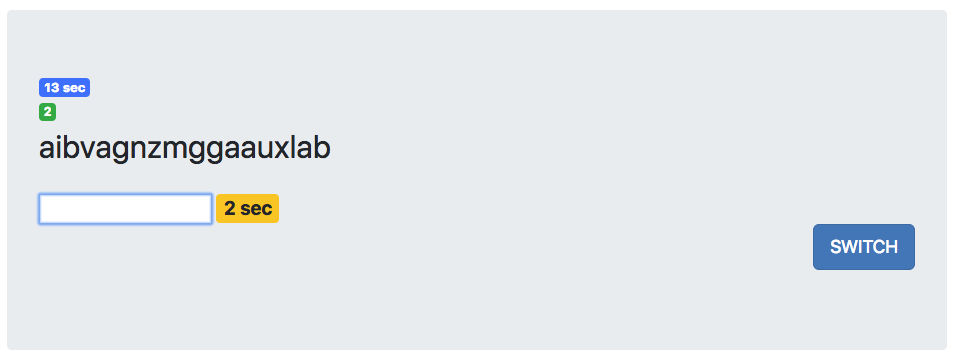
\includegraphics[width=\textwidth]{graphs/screenshot_RET_alone.png}
        \caption{Sample Screen of the Letter Counting Task}
        \label{fig:LC_screen}
    \end{figure}
    
    This particular task was chosen as it fulfills several requirements of my design. First, the main research questions address the effects of inequality on performance measures, like output and efficiency. To be able to observe changes in those measures it is important to ensure that participants are not simply always doing as much as time allows, i.e. a corner solution, but that they choose an optimum based on their personal preferences. Such a phenomenon would be particularly strong if players have a significant intrinsic motivation, or if no incentive is offered to stop solving tasks \citep{frey1997}. An example of a task with a high intrinsic motivation would be any fun game, such as Tetris, for instance.
    The Letter Counting Task is tedious and repetitive without being effortless and therefore is a particularly revealing exercise to determine effort exerted due to monetary incentives \citep{cerasoli2014}.\\
    
    Furthermore, the task is easy to explain and is not mathematical, which has been shown to induce a gender gap in a competitive setting not linked to skill \citep{niederle2010}.\\ 
    
    \subsubsection{Incentivised Leisure}
    \label{ss:switch_mode}
    
    Another issue present when trying to identify work supply levels in the laboratory that might produce a corner solution is the missing incentivisation of non-work. In real life, leisure has an intrinsic motivation which, in economics, is quantified by the opportunity costs of not working. In the laboratory, however, due to the short time frame, implicit peer pressure and possible experimenter demand effects, participants might be reluctant or even opposed to reducing their work input and spending time in leisure. To address this issue, a fundamental feature of my design is, following \citeauthor{sausgruberForthcoming}, the monetary incentivisation of leisure time.\\
    
    In my experiment, participants have, at any point while solving the RET, the opportunity to change to a leisure mode where they are paid per time unit and do not need to work. In this leisure mode, that was called ``switch'' mode to avoid any stigma on shirking \citep{rey-biel2016, eriksson2009}, players obtain 1 token for each 10 seconds they spent in it. A confirmation screen is shown to ensure that participants do not enter the ``switch'' mode by mistake.
    
    \subsubsection{Increasing Difficulty and Optimality}
    
    Depending on a participant's ability, there must exist a rate of payment per time unit for which she or he is indifferent about offering work -- solving the task -- or spending time in leisure mode. Assume, for instance, that a participant needs one second to solve a sequence of given length and earns one monetary unit for that. If he or she would also earn one monetary unit per second in the leisure mode, they would stay in the ``switch'' mode given the disutility of labor. However, if he or she needs less than one second, they would prefer to solve the sequence as they would then earn more. Between those two points, and according to the transitivity and continuity axioms of choice, there must be a point where they were indifferent.\\
    
    In my design, and following the procedure used by \citeauthor{sausgruberForthcoming}, the Letter Counting Task starts at a level so easy that any participant would earn more by solving the task than by spending time in ``switch'' mode. The sequence then increases in length by four characters. With each iteration it becomes more difficult to count the number of ``a''s in the sequence. Depending on their abilities, each player will have a point at which he or she would earn more by staying in the ``switch'' mode. By observing the times taken to solve each task, it is possible to determine the point at which any given participant should have changed to the leisure mode.\\
    
    This difficulty increasing feature is also one of the reasons why I chose the Letter Counting Task. The random sequence is easily generated while the difficulty increase (the length increase) can be easily and quantifiably changed. In fact, it allows for several parameter changes for future research. For instance the speed of increase, the change rate between ``switch'' and task, or the letters that are to be counted.\\
    
    To ensure that the solution to the subsequent sequence is not just the number of letters in the last sequence plus a small number, for each generated sequence a new sample from a new population with a different distribution is drawn. This makes it unviable to just guess the number of ``a''s in the sequence by starting at the count of the last one.
    
        
    \subsection{Learning Effects}
    Since the experiment consists of several benchmarking and competition rounds, it was important to have a task that would present little increase in performance after each repetition. Otherwise, it would have been difficult to compare the outcomes of the baseline and the competition rounds for the same participants.\\
    
    To reduce the impact of learning on the number of tasks solved as the experiment progresses, the task and design selected allow for enough repetition and learning even before the measurements of work supply and investment start. 
    %Moreover, within each round there are several repetitions. On average, a participant solves 11.6 sequences per round. 
    After that, there does not seem to be much room for improvement in recognizing ``a''s after doing it a couple times. Figure \ref{fig:avg_time_task} shows the average time participants of the experiment needed to solve the first 16 tasks across the 8 competitive rounds. Although there is an increase in variance as the task becomes more difficult (going from the top left to the bottom right box), there is no visible decrease in the average time needed by participants to solve each task across rounds (going from left to right in each box).\footnote{Note that this assumes similar learning effects across individuals.} 
    
    \begin{figure}[h]
        \centering
        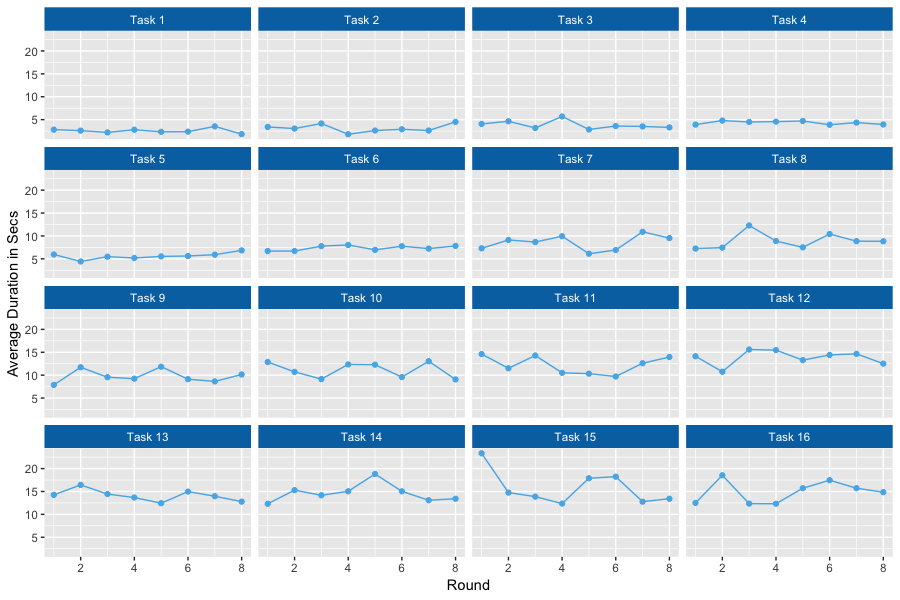
\includegraphics[width = \textwidth]{graphs/avg_time_per_task_round.png}
        \caption{Average Time in Seconds Needed to Solve the First 16 Tasks Across Rounds}
        \label{fig:avg_time_task}
    \end{figure}
    
    
    \subsection{Benchmarking}
    \label{ss:benchmarking}
    
    To identify the levels of performance in a non-competitive environment, two rounds of the RET are played during the introductory section of the experiment. In the first round, participants receive what will be the low piece rate (the payment per sequence if they do not win the previous contest), while in the second they receive the high piece rate (the payment per sequence if they are declared the winner of a period). The latter piece rate was, in my case, double the low piece rate so that a participant would optimally take up to twenty seconds solving a sequence before switching to the leisure mode. The order of the benchmark rounds -- first low, then high piece rate -- was selected to make the difference in earnings more noticeable and significant.
    
    Instructions and control questions were shown before both the low and high piece rate paying benchmarking rounds. In the control questions before the high wage benchmark round, I chose the possible answers such that selecting the correct answer for the low wage benchmark round would be possible, so forcing participants to think why there was a change in the maximizing time to solve sequences. Participants could only advance if they responded correctly to all the control questions (see control questions in section \ref{sec:intro_exp}).
    
    \subsection{Help and Feedback}
    
    During solving of the Real Effort Task (RET) a summarized version of the instructions is shown at the bottom of the page and a mouseover display explains all relevant elements if needed. Once a participant goes into the ``switch'' mode, a counter shows in real time how many tokens he or she earns with each passing second and informs him or her about the number of sequences solved.\\
    
    Finally, a feedback screen shows how many sequences were solved, how much time was spent in the ``switch'' mode, and the total earnings for the round. In the second round of the baseline setting RET, another table informs the participant about the earnings in the previous round to make the difference in earnings, between the high and the low piece rate, more obvious.\footnote{See appendix \ref{ax:screenshots} for an example of the feedback screen.}
    
    \section{Experiment Walkthrough}
    \label{sec:intro_exp}
    
    To start, the introductory section welcomes the participants and informs them about the functioning of the experiment and the RET.
    
    \subsubsection{Real Effort Task Instructions and Trial Round}
    
    After a short welcome to the experiment, participants are told the main goal of the RET (counting ``a''s) and how they submit their answers by typing the correct number in the input field and pressing ``enter'' (see section \ref{sec:RET} for more detail). They then have the opportunity to test the task five times with five different sequences that were chosen to show the variability of the sequences. Some were long and some were short, some had many ``a''s and some had few. When a correct answer is submitted, the next sequence is shown and the current timer is restarted. \\
    
    The screen also featured an annotated tour that explained every part of the RET screen: the sequence, the input field, and a timer counting the number of seconds needed to solve the current and the previous sequence.
    
    \subsubsection{``Switch'' Mode Instructions}
    
    Once participants complete the trial round, they are introduced to the leisure mode, the payment scheme, and the increasing difficulty mechanism of the RET. As explained in more detail in section \ref{sec:RET}, the incentivised leisure mode is a core feature of my experiment. As aforementioned, during the experiment it is called ``switch' mode to avoid any stigma on shirking.\\
    
    Participants are paid one token per correctly solved sequence, with one token being converted to EUR 0.1 at the end of the session. While in the ``switch'' mode, they earn 0.1 tokens per second spent in it. On this screen, I go to great effort to let participants know that, in terms of payment, the ideal point to switch is when he or she takes longer than 10 seconds to solve a sequence, regardless of how much time is left or how many sequences they have solved thus far. However, I do not explicitly define that as the optimum since in the competition rounds it might be advisable to solve more sequences to increase the chances of a higher piece-rate.\\
    
    On this screen, an illustrative example of possible earnings is presented, participants can try the RET several times, and an annotated tour introduces the new elements (a counter showing the total solved sequences, a time countdown, and the switch button).
    
    \subsubsection{Control Questions}
    
    On this page, participants are asked two sets of questions to ensure that they have understood the instructions. As explained in 3.1.3., they must answer all questions correctly to proceed.\\
    
    In the first set, participants are asked how much a fictional player would have earned given an amount of solved sequences and time spent in the ``switch'' mode (Fig. \ref{fig:cq_earnings}). The numbers were chosen so they would not offer an obvious anchor point,\footnote{An anchor point is an amount of time or number of sequences solved that a participant is supposed to aim for while solving the RET.} while still being easy to calculate.\\
    
    \begin{figure}
        \centering
        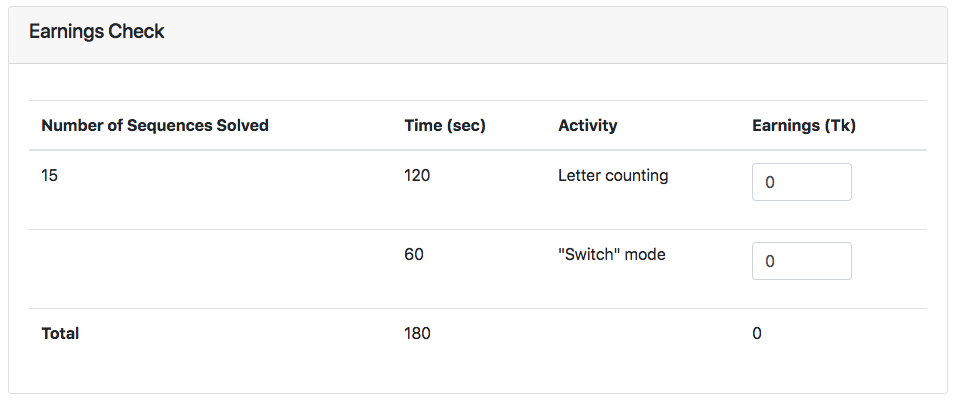
\includegraphics[width=\textwidth]{graphs/cq_earnings.png}
        \caption{Control Question: Earnings}
        \label{fig:cq_earnings}
    \end{figure}
    
    In the second set (Fig. \ref{fig:cq_switch}), participants were asked to select the switching point of a fictional player aiming at maximizing her payoff. Once again, the times were selected in such a form so that a tendency to infer an anchoring point would be minimized. Similarly, instead of giving examples of actual sequences, only a visualization with bars is given.
    
    \begin{figure}
        \centering
        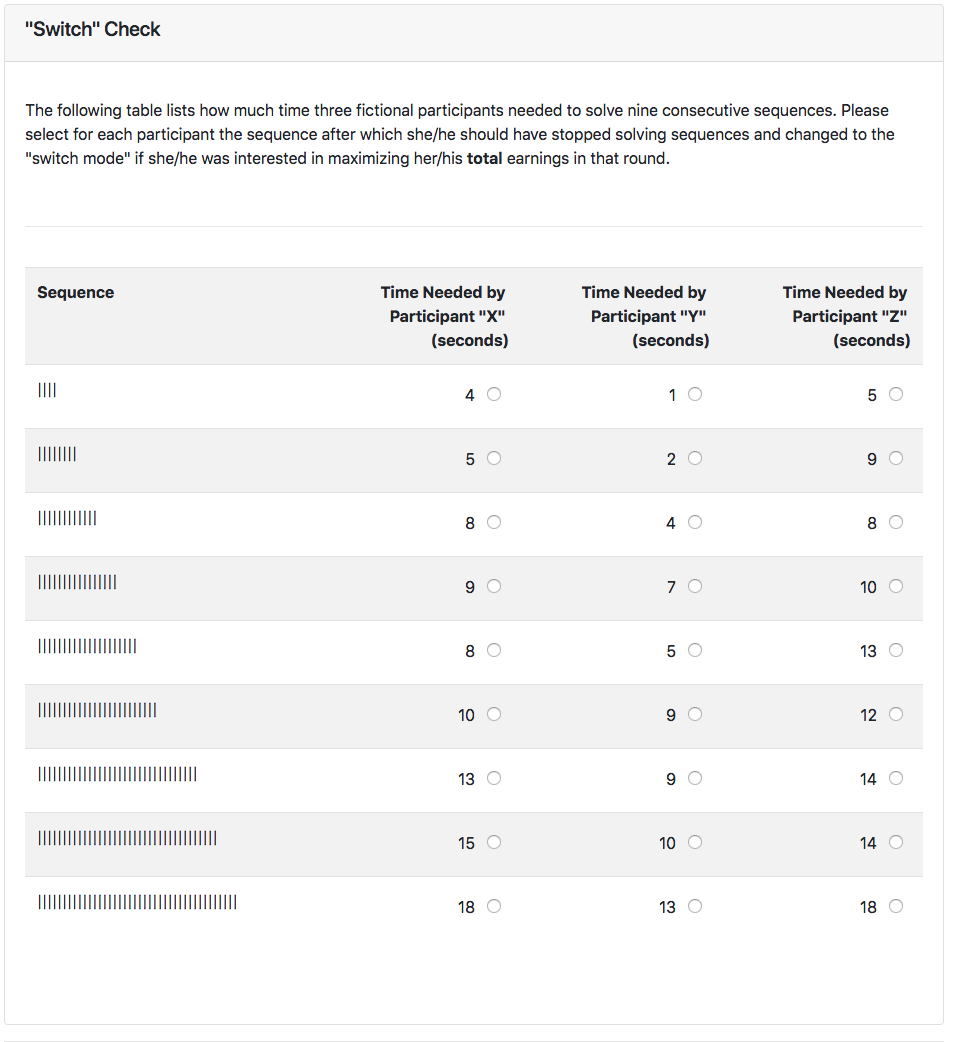
\includegraphics[width=\textwidth]{graphs/cq_switch.png}
        \caption{Control Question: ``Switch'' Mode}
        \label{fig:cq_switch}
    \end{figure}
    
    
    \subsection{Competition Section}
    \label{ss:compt}
    
    At the beginning of the competition section, participants are informed that they were randomly placed into groups of three people and that each person was assigned a label \textit{A, B} or \textit{C}, but that their identity and that of all other participants will remain anonymous both to all other participants as well as to the experimenters.\footnote{This reduces the impact of other-regarding behavior.} I chose groups of three people for the experiment as the group dynamics are more interesting and revealing in the case of three players when compared to two, and this did not increase the modelling complexity too much. With three players it is possible, for instance, to compare competitive behavior between losers in subsequent rounds. Most importantly, it allows me to make a distinction between players \textit{without the highest} possibility of winning and those \textit{with the least} possibility of winning.\\
    
    At the beginning of the competition section, participants in the treatment sessions are further informed about the taxation and redistribution scheme (see section \ref{sec:treat}).\footnote{Note that when moving from the introductory section to the competition, two things change in regard to the RET and the performance incentives. First, the competitive aspect of being in the group. Participants will have the possibility to see what others do and will know that the other participants will see their own performance. In fact, last place aversion and the utility of winning itself have been shown to be the driving issues behind overbidding in rent-seeking contests as well as behind performance increase in competitive games \citep{sheremeta2013}. Second, in the actual contest, increasing one's earnings can also indirectly increase the chances of winning the prize through a larger available income to invest.\\
    The fact that these two factors change at the same time might make it difficult to pin-point reasons behind a performance change between the benchmarking and the competition rounds. This does, however, not affect any of the main variables I am interested in investigating in this study since we can still precisely determine the optimal investment and switching time for each participant and their difference to the observed values. Furthermore, the effects of competition, inequality, impulsiveness, etc. have already been extensively researched, including in the context of rent-seeking contests. In fact, \cite{sheremeta2016} shows that the main factor is impulsiveness, which I control as explained in subsection \ref{ss:CRT}. For these reasons, I do not alter the experiment, but discuss a possible workaround and its drawbacks in chapter \ref{ch:discussion}.} 
    
    \subsubsection{Tullock Contest}
    
    Next, players are informed about the contest proper. In eight rounds, each participant will have the opportunity to earn money by solving the Letter Counting Task or by spending time in the ``switch'' mode. Money earned through work\footnote{I.e. the net income earned by counting letters plus the redistributed amount.} can then be invested to increase the higher piece rate in the following round. Only one person per round is awarded the prize and the probability of winning it is equal to the share of that person's investment relative to all investments by all players. An example for easier understanding is also shown (see the screenshots (e) and (f) in Figure \ref{ax:screenshot_3} in the appendix).\\
    
    Players are further reminded at this stage of how much they earned in the benchmarking rounds and of the difference in earnings between the low and high piece rate rounds. Note that every time before the Real Effort Task (RET) starts, a waiting page makes sure that all participants have completed all previous sections, thus avoiding some participants solving the task while others are reading. Also, a confirmation page is displayed before the start of the RET so that participants are not taken by surprise.
   
    \subsubsection{Beliefs}
    
    To test if, and to what extent, players take the behavior of the others into account when choosing their production and investment levels, beliefs about the production, i.e. the number of sequences solved, and the amount invested by the other team members are gathered in every round. A visual clue lets them know which player has a higher piece rate in the current round.
    
    \subsubsection{Feedback and Result}
    
    After solving the task (as explained in section \ref{sec:RET}) and before investing, participants receive feedback on their performance like they did in the benchmarking section. They are provided a summary of: how many sequences were solved, how many seconds spent in ``switch'' mode and, in the case of the treatment, how much the transfers are.\\
    
    After the investment, participants receive detailed feedback about the investments and performance of the group and are informed about who won the high piece rate in the following round (see Fig. \ref{fig:screen_results}).
    
    \begin{figure}[h!]
        \centering
        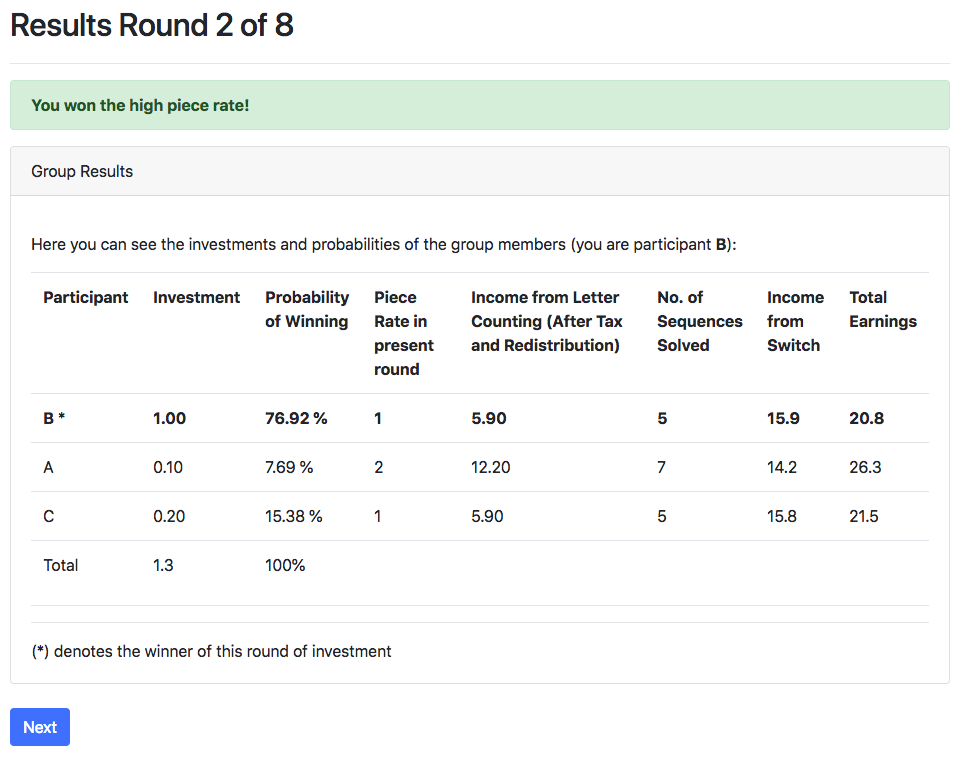
\includegraphics[scale = 0.4]{graphs/screen_results.png}
        \caption{Results Screen after Investment}
        \label{fig:screen_results}
    \end{figure}
    
    \vspace{-2mm}
    
    \subsubsection{Investment}
    
    On the investment screen, players use a slider to choose their investment in steps of 0.1 tokens. They are informed about their total available income for investment, how much they invest, how much they would keep, and what the prize is. They are also reminded that tokens invested are not refunded, even if the prize is not awarded (see Fig. \ref{fig:screen_invest}).
    
    \begin{figure}[h!]
        \centering
        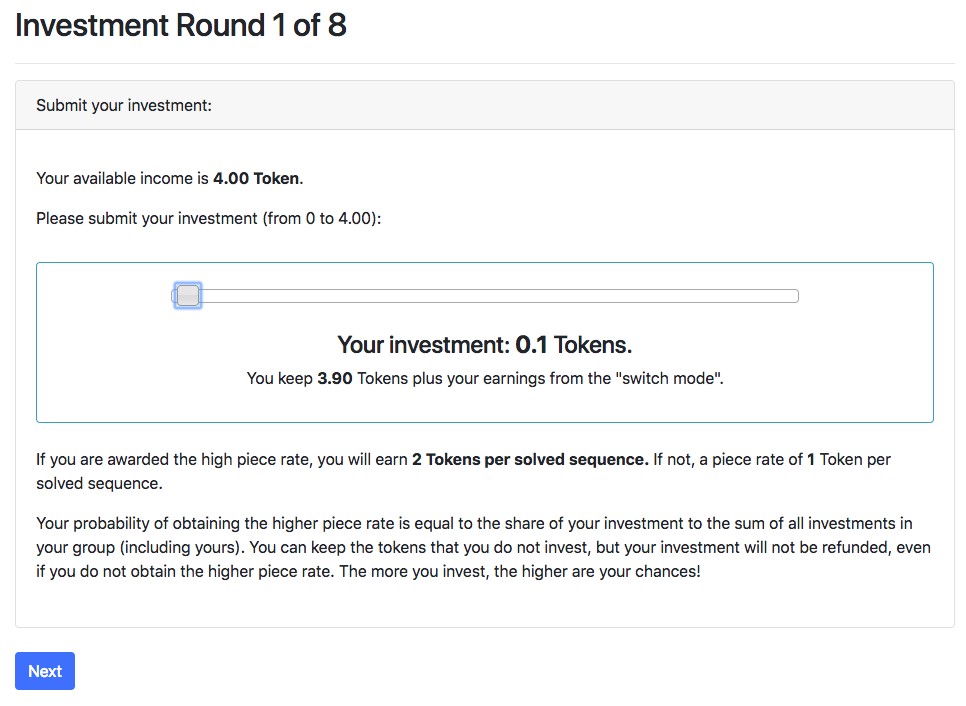
\includegraphics[scale = 0.4]{graphs/screen_invest.png}
        \caption{Investment Screen}
        \label{fig:screen_invest}
    \end{figure}
    \vspace{-2mm}
    
    \subsection{Treatment: Taxation and Redistribution of Income}
    \label{sec:treat}
    
    As explained in the introduction to this thesis, understanding how voting would affect the POUM itself requires several layers of examination. In the present work, I look at how the general dynamics of the contest behave and what impact taxation and redistribution have on the distribution of win probabilities and the exertion of effort.\\
    
    To test this, I introduced a treatment where income from work, that is, from counting letters but not from ``switch'' mode, is taxed at 60\%. The entire tax revenue is then divided equally among all participants so that the total amount of tokens in circulation is constant. Participants can then invest their net income plus transfer to increase their chances of earning the higher piece rate, as explained in section \ref{ss:compt}.\\
    
    In the control group there is no taxation and therefore no redistribution. The available income to invest is exactly equal to the earned tokens from letter counting. Note that the predictions regarding the optimal investment, as derived in chapter \ref{ch:model}, are unchanged since taxation and redistribution only affect work income. However, taxation does affect the valuation of the game where $\mathbb{V}$ is no longer equal to just the difference in earnings between the high and low wages, but adds the share of the sum of redistributed income $R$ such that $\mathbb{V}_i = x_{hw}*w_{hw} - x_{lw}*w_{lw} + \frac{R}{n}$.\footnote{Here, x is the amount of sequences solved, $w$ the paid piece rate, and $hw$ demarks the high and $lw$ the low wages.}  
    
    \subsubsection{Taxed Benchmarking}
    \label{ss:tax_bench}
    
    To more effectively measure the valuation of the price in the taxation treatment, two extra rounds paying a wage equal to the effective taxation in the treatment were added to the benchmarking phase for the treated group, as explained in subsection \ref{ss:benchmarking}.\\
    
    Specifically, in between the low piece rate and high piece rate benchmarking another benchmark round was introduced. This round paid, per task, the equivalent of the effective taxed low piece rate after redistribution or $w(1-t)+ w(t/n)$,\footnote{If the total tax revenue is divided in equal parts among all individuals, as is the case in my design.} with $w$ being the piece rate, $t$ the tax rate and $n$ the number of players per group. In my case, this means 0.6 tokens per sequence or 1 token minus 40\% of 1. The payment for the ``switch'' mode remained, as in all rounds, constant.\\
    
    Similarly, an extra round was introduced after the high wage round which paid the equivalent of the effective taxed high piece rate after redistribution, in this case this was 1.2 tokens or 2 tokens minus 40\% of 2. These extra rounds were introduced in this order so as not to generate a strong separation between the taxed and the untaxed rounds, as well as to space out the control questions. \\ 
    
    To ensure that introducing these extra rounds did not affect the participants' performance, I carried out a Wilcoxon test between the productions of the treated and non-treated groups. This was done once for the low benchmark and once for the high piece rate benchmarking rounds. Both showed no differences between the groups, i.e., no learning or timing effects, nor a significant difference in skill. The test results are summarised in the appendix in table \ref{tab:bench_prods_test}.
    
    \subsection{Idiosyncratic Controls}
    
    To control the effect of idiosyncrasies, like risk aversion, on players' behavior, I introduced several tests at the end of the experiment which are presented in this section. 
    
    \subsubsection{Fairness Sentiment}
    
    To see how participants themselves perceived the game in terms of what determined success, they were asked to rate from 0 to 7 what determined their success in the game. With 0 being only luck and 7 being only skill. Figure \ref{fig:fair_q} shows the voting screen. The question was posed both at the beginning and end of the competition. Allowing us to observe not only how the perception changes after experiencing the competition, but if, and to what extent, the fairness perception changes in the presence of redistribution.\\
    
    This measure can, furthermore, be useful in comparisons with other designs and parametrizations as discussed in chapter \ref{ch:discussion}.
    
    \begin{figure}
        \centering
        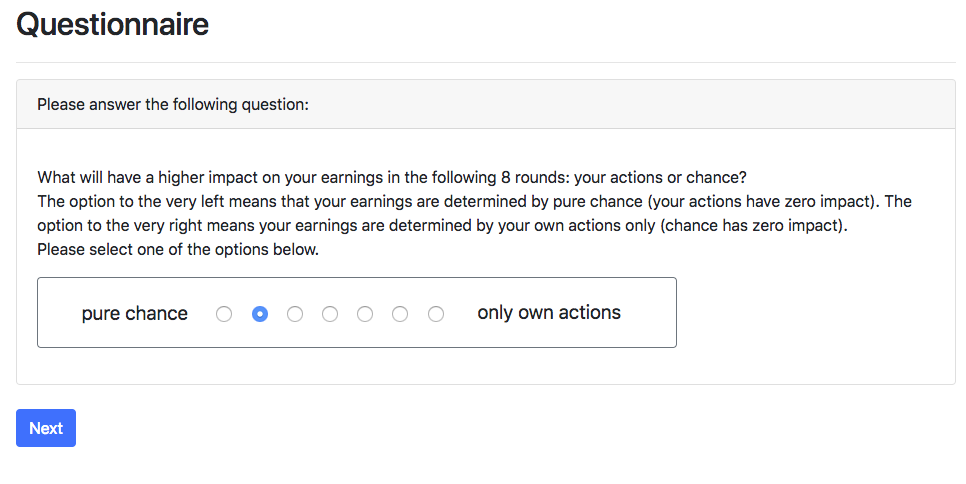
\includegraphics[width=\textwidth]{graphs/Fairness_Q_Begin.png}
        \caption{Screen Fairness Questionnaire (beginning)}
        \label{fig:fair_q}
    \end{figure}
    
        
    \subsubsection{Risk Aversion Measure and Risk Elicitation}
    
    During the investment section of the experiment players participate, effectively, in a lottery. The exact terms of that lottery are not known to them in advance and present a strategic decision as well. Their investment choices will therefore not only reflect their strategic considerations, but also their stance on risk taking.\\
    
    To control the effect of this, I include an incentivised risk elicitation test following the \textit{Multiple Price List} by \cite{holt2002} (HL) with the implementation for \textit{oTree} taken from \cite{holzmeister2017}.\\
    
    I chose the HL method as it, according to \cite{crosetto2016} and \cite{harrison2008}, among other reasons:
    \begin{itemize}
        \item allows for risk preferences in both the risk neutral and risk seeking range;
        \item has a finer categorisation as for instance \cite{eckel2008};
        \item has constant intervals between the parameters of risk, mapped through discrete choices, which makes it robust against stochastic decision making;
        \item does not strongly differentiate between genders -- there are no significant differences between genders.
    \end{itemize}  
       
     In the HL method, players are asked to choose between several pairs of lotteries, A and B. Beginning with a choice where option A is the safer choice, the last choice is between sure outcomes, where B represents the payoff maximizing choice. Between them, there is a point where a participant changes from one option to the other, thus revealing his or her risk preferences.\\
     
     Figure \ref{fig:choices_mpl} shows the list of choices that participants were presented with. In it, probabilities are visualized with the help of pie charts and all possible decisions are shown at once. Consistent preferences were forced to avoid elimination of data in the already small sample. After choosing, one of the decisions was then selected randomly and the lottery drawn and paid out.\\
     
     \begin{figure}
         \centering
         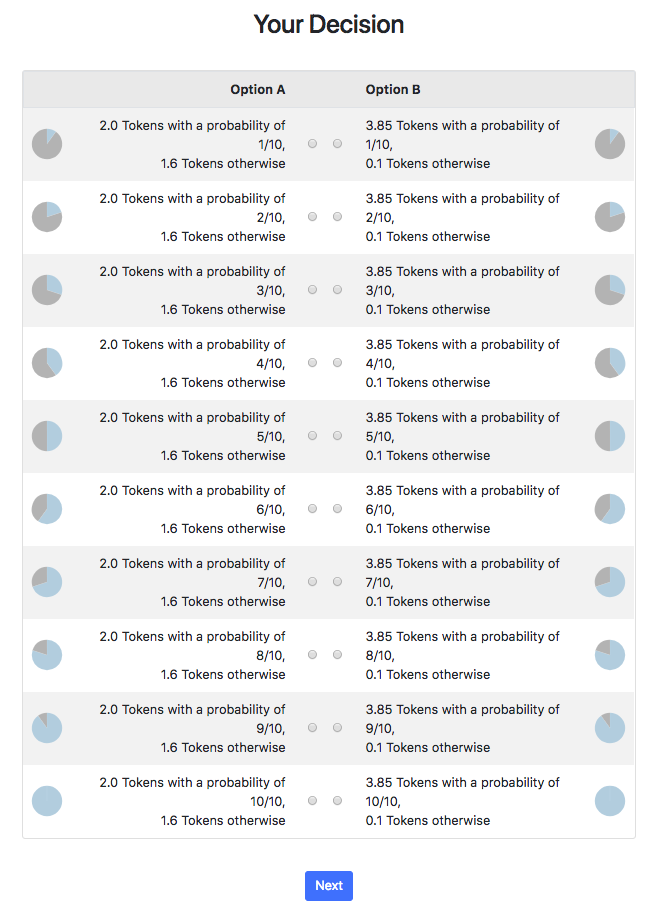
\includegraphics[scale=0.4]{graphs/Choices_MPL.png}
         \caption{Choices Screen \textit{Multiple Price List}}
         \label{fig:choices_mpl}
     \end{figure}
     
     
    Following the common procedure, I assume participants to have a constant relative risk aversion (CRRA) utility function $u(x)=x^{(1-r)}$, which allows me to index each choice by a corresponding $r$. An individual with an $r<0$ is categorized as risk averse, with $r=0$ as risk neutral, and with $r>1$ as risk seeking. The payoffs are exactly the same as those used by \cite{holt2002} and thus imply that someone switching after the fourth lottery to \textit{option B} is assigned an $r$ interval of (-0.15, 0.15), meaning risk neutrality. The list of the implied risk aversion ranges can be seen in table \ref{table:HL}, where the number of safe choices is the number of choices made before switching to \textit{option B}.
    
    
    \begin{table}[]
    \centering
    \begin{tabular}{lll}
    \hline
    \hline
    \begin{tabular}[c]{@{}l@{}}Number of \\ Safe Choices\end{tabular} & \begin{tabular}[c]{@{}l@{}}Range of Relative\\ Risk Aversion\end{tabular} & \begin{tabular}[c]{@{}l@{}}Risk Preference \\ Classification\end{tabular} \\
    \hline
    0-1                                                               & r < -0.95                                                                 & Highly Risk Loving                                                        \\
    2                                                                 & -0.95 < r < -0.49                                                         & Very Risk Loving                                                          \\
    3                                                                 & -0.49 < r < -0.15                                                         & Risk Loving                                                               \\
    4                                                                 & -0.15 < r < 0.15                                                          & Risk Neutral                                                              \\
    5                                                                 & 0.15 < r < 0.41                                                           & Slightly Risk Averse                                                      \\
    6                                                                 & 0.41 < r < 0.68                                                           & Risk Averse                                                               \\
    7                                                                 & 0.41 < r < 0.97                                                           & Very Risk Averse                                                          \\
    8                                                                 & 0.41 < r < 1.37                                                           & Highly Risk Averse                                                        \\
    9-10                                                              & 1.37 < r                                                                  & Stay in Bed\\
    \hline
    \end{tabular}
    \caption{Risk Aversion Classifications Based on Lottery Choices\\ \citep{holt2002}}
    \label{table:HL}
    \end{table}
    
    \subsubsection{Cognitive Reflection Test}
    \label{ss:CRT}
    
    A tendency to overbid in rent-seeking contests has been well documented \citep{sheremeta2013, dechenaux2015}. This is particularly critical to consider in my design, as overbidding, both in terms of work supply and investment, would be interpreted as an over-exertion of effort.\\
     
    While there are several proposals as to what influences this behavior, \cite{sheremeta2016} suggests that impulsiveness might be the strongest predictor. In fact, he suggests that, when analyzed simultaneously with the utility of winning, systematic biases, relative payoff maximization, and mistakes, only impulsiveness remains statistically significant.\\
    
    Following his work I therefore include a Cognitive Reflection Test based on \cite{thomson2016}. They propose alternative questions to measure cognitive reflection that are less well known as those originally posed by \cite{frederick2005}. Figure \ref{fig:crt_quest} shows the questions that were presented to participants, although these were presented individually and without the possibility to go back, instead of all at once.
    
    \begin{figure}
        \centering
        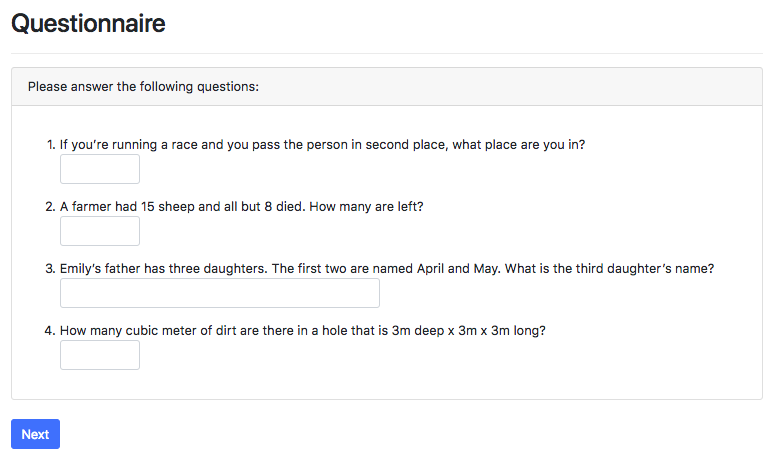
\includegraphics[width=\textwidth]{graphs/CRT_Quest.png}
        \caption{Cognitive Reflection Test \citep{thomson2016}}
        \label{fig:crt_quest}
    \end{figure}
    
    \section{Hypotheses}\label{sec:hyp}
    
        
    
%\textcolor{red}{Be sure to reference to the \textit{quantal response equilibrium} (QRE) developed by \cite{mckelvey1995} and the result in \cite{sheremeta2011} in the hypothesis study. explain how QRE (Sheremeta 2011) can influence the results in our experiment. Note that we have larger groups and variable endowments. check this with our hypotheses}\\


%\textcolor{red}{Be sure to reference to the results in \cite{fallucchi2017} in the hypothesis study. explain which type of inequality applies in our experiment. What is the expected behavior. check this with our hypotheses. May be even expand on the study and its results. Sound very consequential and similar to what its being done in the thesis}\\
    
    
    I focus in this thesis on the dynamic of repeated Tullock Contests, in particular on the participants' tendency to over-invest, and the evolution of winning probabilities across periods. As explained in the introduction, those probabilities can be seen as analogous to the Prospect of Upward Mobility while the investments made in each round are analogous to investments made in human capital needed to acquire high earning jobs.\\
    
    Broadly speaking, my thesis looks at performance values in terms of sequences solved and time spent in leisure mode, and at effort exertion values in form of investments. Comparisons in those regards are made both within and between subjects and groups. Within subjects and groups, I look at the differences between the benchmark and the competitive rounds in general, and within the competition rounds over time. In addition, I introduce a taxation and redistribution intervention which will be studied through a between-subject and group comparison.\\
    
    How investments develop across periods is the first step to analyze the POUM in my experiment. How much participants invest ultimately determines their probability of winning but, more importantly, it determines the total welfare of the group. Since available income invested is not reimbursed, investments reduce overall welfare. An intervention that reduces over-investment, whilst ensuring winning probabilities that are more fair\footnote{The definition and analysis of the concept of fairness go far beyond the scope of the present thesis but these are addressed in chapter \ref{ch:conclusion} as part of the discussion.} is therefore desirable.\\
    
    As described in the model in chapter \ref{ch:model}, investments should, in theory, be constant over time, however, as \cite{sheremeta2016}, among others, have shown, participants tend to over-invest. I expect, nevertheless, that over-investment decreases over time, due to income effects or because they develop a better knowledge of the game. This phenomena is shown experimentally by \cite{fallucchi2013} where, although investment levels stay above optimum, they clearly drop in the presence of full information, as is the case in my design. In that experiment, groups with full information reduced over-investment to around 13\% above optimum while those with only feedback about their own performance stayed at levels of 66\% above optimum. Formally, I expect, therefore, that:
    
     \begin{hyp} \label{hyp:treat}\textit{Mean investments will be higher than the expected profit maximizing value for all treatments, but will decrease over time.}\end{hyp}
     
    As it has been described in the literature on rent-seeking contests, over-investment can be driven by several aspects, most importantly, impulsiveness, risk incline, competitiveness and inequality aversion. I control risk aversion and impulsiveness with the methods mentioned above in the experimental design section (Cognitive Reflection Test and Multiple Price Listing). Furthermore, if competitiveness plays a major role I should observe no major difference between treatments or over time. Considering the second part of hypothesis \ref{hyp:treat}, that not only do I expect investments to be higher than optimal but to decrease over time, if that decrease is driven mainly by a better understanding of the game or better knowledge of other participant's behaviour, I should not observe any difference in slope between treatments. In the latter case, I would further expect an increase in the accuracy of a participant's belief about the investment \textit{and} performance (since performance determines the valuation) of the group's other participants.\\
    
    On the other hand, the reduction in investments effect can be driven by an income effect, since in each period only one person wins but two lose. If winners of previous rounds are more likely to invest more and therefore also more likely to win again, losers might invest less each time.  In this case, I should observe a significant difference between winners and losers and a significant effect of cumulative wins on the invested amount.\\
    
    Another possibility as to why mean investments will decrease over time is that participants have a decreasing utility function for winning. In other words, that participants value winning the first round higher than winning the last one. My design does not disentangle this effect from experience effects, yet this issue is discussed for further research in chapter \ref{ch:conclusion}.\\
    
    In case inequality aversion is a driving factor in competition, introducing a redistribution scheme should reduce its effect as income distributions within groups become more equal. Additionally, given that the available income is more equally distributed in the treatment by design I expect investments in the taxed groups to be relatively lower. Formally:
    
    \begin{hyp} \label{hyp:treat-overinvest}
    \textit{Participants in the taxation treatment will invest a smaller multiple of their optimal investment.}
    \end{hyp}
    
    In other words, participants in the treatment group will be relatively closer to their optimal investments. Note that the compared measure is the ratio over the optimum since the optimal value of investment is different for both groups. This is because the valuation of the game, i.e. the difference in net earnings between the high and the low wage, is different for each treatment.\\ 
      
    An important corollary of \cref{hyp:treat-overinvest} is that, since players in the taxation treatment are closer to the optimum levels of investment, total welfare for the group in terms of total income generated is larger.\\
    
    Now, what does the expected lower over-investment for the treatment and the decreasing investments over time mean for the probability of winning? In other words, how do investments change relatively to the other group members in the cross-sectional and longitudinal dimensions?\\
    
    If investments decrease over time mainly due to subject specific differences (learning, decreasing utility of winning, etc.), I should not observe any significant differences between treatments or over time with regard to the distribution of probabilities since the bids decrease equally for all subjects. If, however, the effect is driven by group dynamics, for instance last place aversion or income effects of cumulative wins, I expect to see a stronger variance in probabilities in the control group while increasing over time. In the redistribution treatment, available income will be more equally distributed and therefore inequality and income effects should be diminished. In other words, probabilities will be closer to each other and to the mean of $1/n$. Formally:
    
    \begin{hyp}\label{hyp:wins}
    \textit{The coefficient of variation of winning probabilities will be increasing across rounds while being smaller in the treatment group.}
    \end{hyp}
    
I use the coefficient of variation $c_v=\frac{\sigma}{\mu}$ to test if the distribution of probabilities between the treatments really differ, as for instance in \cite{rassenti2000}, as \cite{bendel1989} recommends to use this in cases where there is a relatively exact measure of the values, although given the fact that the mean of the probabilities is always equal to $1/n$ the results correspond to the standard deviation of each sample.
 